\chapter{Oscilador Controlado por Tensión (VCO)}
\section*{Resumen}
En este capítulo se presenta el diseño, simulación, fabricación y caracterización experimental del módulo del oscilador controlado por tensión (VCO), bloque encargado de generar la señal de microondas en la banda de operación del radar FMCW. Se justifica la selección de los componentes, el diseño de la placa de circuito impreso y, finalmente, se contrastan las simulaciones con las mediciones.

\section{Introducción}
El oscilador controlado por tensión es el componente encargado de convertir la tensión de control en la frecuencia de salida del lazo. Para garantizar el correcto funcionamiento del radar FMCW, el oscilador debe presentar una cobertura de frecuencia adecuada para el barrido requerido ($1{,}55~\mathrm{GHz}$ a $1{,}85~\mathrm{GHz}$), una potencia de salida suficiente para excitar tanto el divisor de potencia como la etapa de realimentación, y una adecuada pureza espectral.

A continuación se detalla la selección del componente comercial adoptado, los cálculos analíticos y electromagnéticos para la adaptación de impedancias en tecnología CPWG, el proceso de fabricación del circuito impreso y la caracterización experimental del bloque en banco de pruebas.

\section{Diseño}

Para cumplir con los requerimientos de ancho de banda y estabilidad exigidos en el sistema de radar FMCW, se ha optado por la utilización del modelo comercial \textit{CVCO55BE-1530-2700} \cite{crystekVCO} de Crystek Corporation, el cual se encuentra entre los dispositivos recomendados por las herramientas de diseño y simulación de RF de Analog Devices (\textit{ADIsimPLL}). Además, este componente presentaba un precio accesible para el laboratorio y se encontraba disponible en Digi-Key.

Los parámetros más importantes de este VCO son los que se muestran en la Tabla~\ref{tab:vco_specs}.

\begin{table}[h]
\centering
\resizebox{\textwidth}{!}{%
\begin{tabular}{|l|c|c|c|c|}
\hline
\textbf{Parámetro} & \textbf{Mínimo} & \textbf{Típico} & \textbf{Máximo} & \textbf{Unidades} \\ \hline
Frecuencia Inferior & - & - & 1530 & MHz \\ \hline
Frecuencia Superior & 2700 & - & - & MHz \\ \hline
Tensión de Sintonía ($V_{\text{tune}}$) & 0.5 & - & 10.5 & VDC \\ \hline
Tensión de Alimentación & 4.75 & 5.0 & 5.25 & VDC \\ \hline
Potencia de Salida & +3.0 & +7.0 & +11.0 & dBm \\ \hline
Supresión de Armónicos ($2^{\text{da}}$) & - & -15 & - & dBc \\ \hline
Sensibilidad de Sintonía & - & 140 & - & MHz/V \\ \hline
Impedancia de Carga & - & 50 & - & $\Omega$ \\ \hline
Capacitancia de Entrada & - & - & 50 & pF \\ \hline
\end{tabular}%
}
\caption{Especificaciones técnicas del VCO Crystek CVCO55BE-1530-2700 \cite{crystekVCO}.}
\label{tab:vco_specs}
\end{table}

La justificación técnica de su selección se fundamenta en los siguientes aspectos clave:
\begin{itemize}
    \item \textbf{Rango de Sintonización y Cobertura de Frecuencia:} El dispositivo opera en un rango de frecuencias que abarca desde los 1530~MHz hasta los 2700~MHz, lo que permite cubrir el ancho de banda de barrido de 1550~MHz a 1850~MHz.
    \item \textbf{Compatibilidad con el Sistema de Control:} Presenta una tensión de sintonización ($V_{\text{tune}}$) comprendida entre 0.5~V y 10.5~V, un parámetro adecuado ya que la alimentación del PLL es de 5~V y para el rango de frecuencias elegido es posible barrer todo el ancho de banda con una tensión de control menor a 5~V.
    \item \textbf{Alimentación compatible con el PLL:} Como su alimentación es de 5~V no es necesario agregar otra alimentación distinta a la del PLL, lo que simplifica la etapa de continua del sistema.
\end{itemize}

Para el diseño de la placa de circuito impreso del VCO se consideró como requisito principal mantener una impedancia de salida de $50~\Omega$.

Para asegurar una alimentación estable, se incorporó un capacitor de desacople próximo al terminal de alimentación del VCO, con el objetivo de reducir el ruido presente en la línea de alimentación. Además, se prestó especial atención a la adaptación de la salida de RF, considerando las características del encapsulado del VCO y del sustrato FR-4 utilizado en la placa.

Finalmente, se incorporaron conectores SMA para la salida de RF y para la tensión de sintonización ($V_{\text{tune}}$), facilitando la conexión con el resto del sistema y la posterior caracterización experimental.

En la Figura~\ref{fig:pinoutvco} se presenta el \textit{pinout} del dispositivo utilizado como referencia para el diseño de la placa.

\begin{figure}[H]
    \centering
    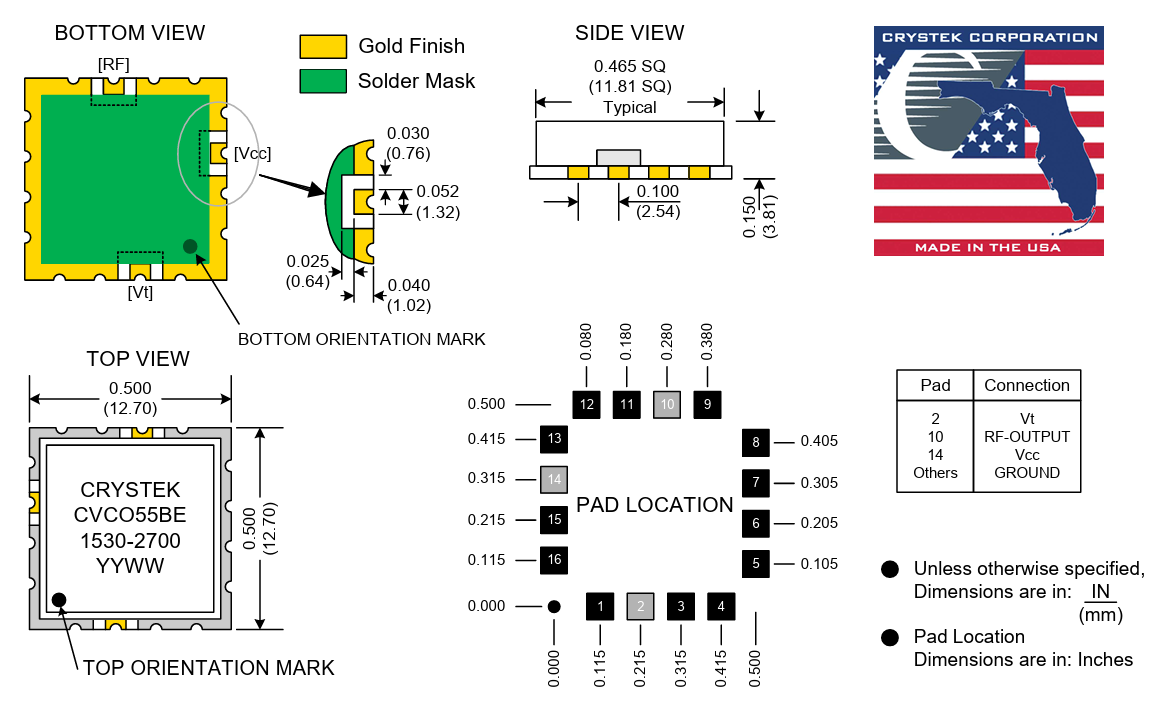
\includegraphics[width=0.75\linewidth]{imagenes/pinoutvco.png}
    \caption{Pinout de referencia. (Fuente: \cite{crystekVCO}).}
    \label{fig:pinoutvco}
\end{figure}

Los valores medidos del sustrato utilizado para realizar el diseño del PCB se muestran en la Tabla~\ref{tab:fr4_specs}.

\begin{table}[H]
\centering
\begin{tabular}{lc}
\hline
\textbf{Parámetro} & \textbf{Especificación} \\
\hline
Material & FR-4 \\
Permitividad relativa ($\varepsilon_r$) & $4{,}3$ \\
Espesor del sustrato ($H$) & $1{,}55~\mathrm{mm}$ \\
Espesor del cobre ($T$) & $0{,}033~\mathrm{mm}$ \\
Tangente de pérdidas ($\tan\delta$) & $0{,}01$ \\
\hline
\end{tabular}
\caption{Parámetros del sustrato FR-4 utilizado para el diseño del PCB.}
\label{tab:fr4_specs}
\end{table}

Se propuso el uso de líneas de transmisión coplanares con plano de masa inferior (CPWG), ya que permiten disminuir el ancho de la pista y las pérdidas. Utilizando la herramienta LineCalc de ADS se obtuvo el ancho de pista necesario para poder desarrollar el proyecto en línea de transmisión coplanar.

\begin{figure}[H]
    \centering
    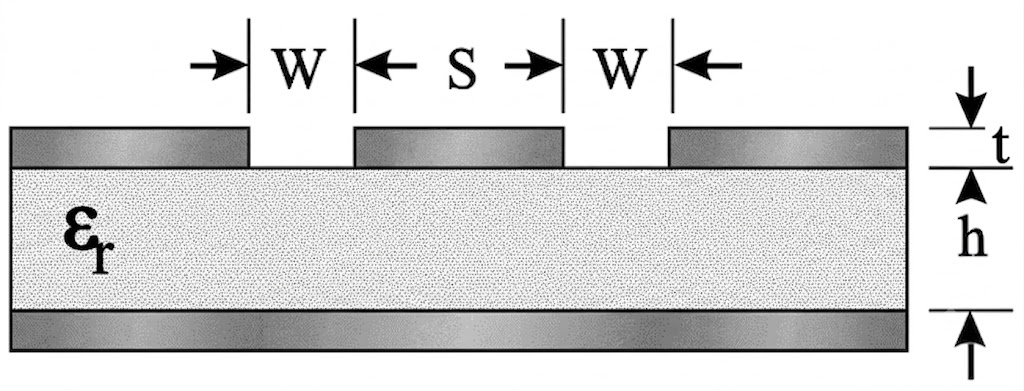
\includegraphics[width=0.65\linewidth]{imagenes/coplanarwgd.png}
    \caption{Línea de transmisión coplanar. (Fuente: \cite{Chemandy}).}
    \label{fig:coplanarwgd}
\end{figure}

Los resultados obtenidos son los siguientes:
\begin{table}[H]
\centering
\begin{tabular}{lc}
\hline
\textbf{Parámetro} & \textbf{Resultado} \\
\hline
Tipo de línea & CPWG \\
Impedancia característica & $50~\Omega$ \\
Frecuencia de diseño & $1{,}7~\mathrm{GHz}$ \\
Ancho de conductor ($S$) & $2{,}61~\mathrm{mm}$ \\
Separación a masa ($G$) & $1{,}00~\mathrm{mm}$ \\
\hline
\end{tabular}
\caption{Resultados del diseño de la línea de transmisión de RF.}
\label{tab:linea_rf}
\end{table}

Para realizar la transición entre el terminal de salida del VCO y la línea de transmisión CPWG de $50~\Omega$, se diseñó una transición gradual mediante un \textit{taper}. El pad de salida del dispositivo presenta un ancho de aproximadamente $1{,}32~\mathrm{mm}$, mientras que el ancho requerido para la línea de transmisión es de $2{,}61~\mathrm{mm}$.

Por último, como indica \cite{HansRosenbergVias}, para ubicar las vías se consideró una frecuencia máxima de operación:

\begin{equation}
f_{\max} = 1{,}7~\mathrm{GHz} + \frac{300~\mathrm{MHz}}{2} = 1{,}85~\mathrm{GHz}.
\end{equation}

Considerando la permitividad efectiva obtenida para la línea CPWG, $\varepsilon_{\mathrm{eff}} \approx 3{,}008$, la longitud de onda guiada resulta:

\begin{equation}
\lambda_g = \frac{c}{f_{\max}\sqrt{\varepsilon_{\mathrm{eff}}}} \approx 93{,}4~\mathrm{mm}.
\end{equation}

Como criterio de diseño, se consideraron separaciones máximas entre vías de $\lambda_g/10$ y $\lambda_g/20$, obteniéndose:

\begin{equation}
\frac{\lambda_g}{10} \approx 9{,}34~\mathrm{mm}
\end{equation}

y

\begin{equation}
\frac{\lambda_g}{20} \approx 4{,}67~\mathrm{mm}.
\end{equation}

Se adoptó el criterio de $\lambda_g/20$, resultando una separación máxima entre vías de aproximadamente $4{,}7~\mathrm{mm}$.

%------------------------simulaciones-----------------------------

A partir de la hoja de datos del VCO Crystek CVCO55BE-1530-2700 se analizó la curva de frecuencia de salida en función de la tensión de sintonización ($V_{\text{tune}}$). El objetivo fue determinar los valores de tensión de control correspondientes al rango de frecuencias requerido por el generador de chirp, comprendido entre $1550~\mathrm{MHz}$ y $1850~\mathrm{MHz}$.

Los valores de $V_{\text{tune}}$ se obtuvieron mediante la lectura de la curva proporcionada por el fabricante, considerando las frecuencias inicial y final del barrido. Estos valores permiten estimar el rango de tensión que deberá proporcionar el lazo PLL para realizar el barrido de frecuencia requerido.

\begin{table}[h]
\centering
\begin{tabular}{lc}
\hline
\textbf{Frecuencia} & \textbf{$V_{\text{tune}}$} \\
\hline
$1550~\mathrm{MHz}$ & $1{,}5~\mathrm{V}$ \\
$1700~\mathrm{MHz}$ & $2{,}7~\mathrm{V}$ \\
$1850~\mathrm{MHz}$ & $3{,}6~\mathrm{V}$ \\
\hline
\end{tabular}
\caption{Valores de tensión de sintonización obtenidos de la hoja de datos del VCO.}
\label{tab:vtune_datasheet}
\end{table}

A partir de los valores obtenidos en la Tabla~\ref{tab:vtune_datasheet} se calculó la sensibilidad de sintonía del VCO, definida como la variación de frecuencia de salida por unidad de variación de la tensión de control. Considerando el rango completo de operación, se obtiene:

\begin{equation}
K_V = \frac{\Delta f}{\Delta V_{\text{tune}}}.
\end{equation}

La variación de frecuencia correspondiente al barrido es:

\begin{equation}
\Delta f = 1850 - 1550 = 300~\mathrm{MHz},
\end{equation}

mientras que la variación de la tensión de sintonización resulta:

\begin{equation}
\Delta V_{\text{tune}} = 3{,}6 - 1{,}5 = 2{,}1~\mathrm{V}.
\end{equation}

Por lo tanto, la sensibilidad de sintonía promedio del VCO en el rango de frecuencias analizado es:

\begin{equation}
K_V = \frac{300~\mathrm{MHz}}{2{,}1~\mathrm{V}} \approx 142{,}86~\mathrm{MHz/V}.
\end{equation}

El valor obtenido resulta cercano al valor típico de $140~\mathrm{MHz/V}$ especificado por el fabricante.

\section{Simulaciones}

Con el objetivo de verificar el funcionamiento del VCO y validar las decisiones de diseño adoptadas, se realizaron diferentes simulaciones previas a la implementación física del circuito.

También se verificó el comportamiento de la línea de transmisión CPWG utilizada para conectar la salida de RF del VCO. El diseño se realizó para una impedancia característica de $50~\Omega$ y una frecuencia central de $1{,}7~\mathrm{GHz}$.

Los parámetros geométricos obtenidos mediante LineCalc fueron utilizados como referencia para la implementación de la placa, considerando un ancho de conductor de $2{,}61~\mathrm{mm}$ y una separación respecto de los planos de masa de $1{,}00~\mathrm{mm}$.

Los parámetros $S_{11}$ y $S_{21}$ luego de la optimización del esquemático fueron los siguientes:

\begin{figure}[H]
    \centering
    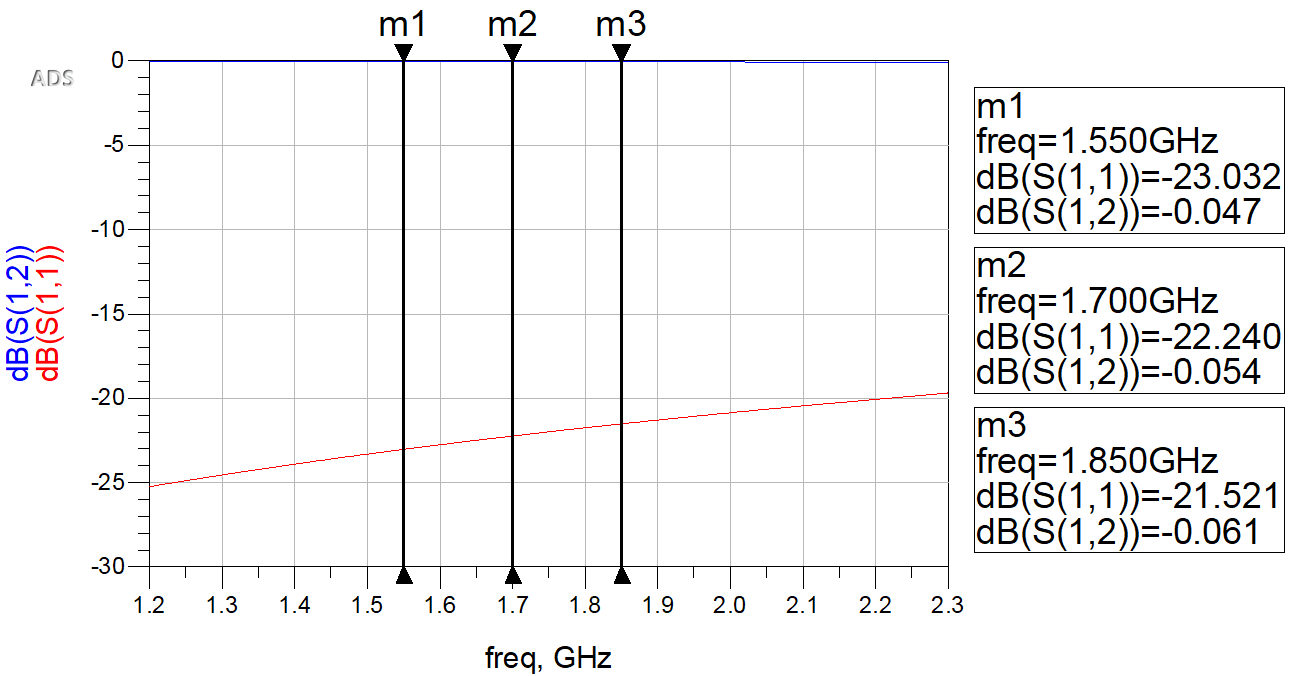
\includegraphics[width=0.75\linewidth]{imagenes/s11s22schvco.png}
    \caption{Simulación del esquemático de la línea de transmisión CPWG de $50~\Omega$. (Fuente: propia).}
    \label{fig:simulacion_linea_sch_vco}
\end{figure}

Para el agregado de las vías se utilizó el layout generado a partir del esquemático anterior, cuya simulación y optimización dieron por resultado la siguiente respuesta de los parámetros $S_{11}$ y $S_{21}$:

\begin{figure}[H]
    \centering
    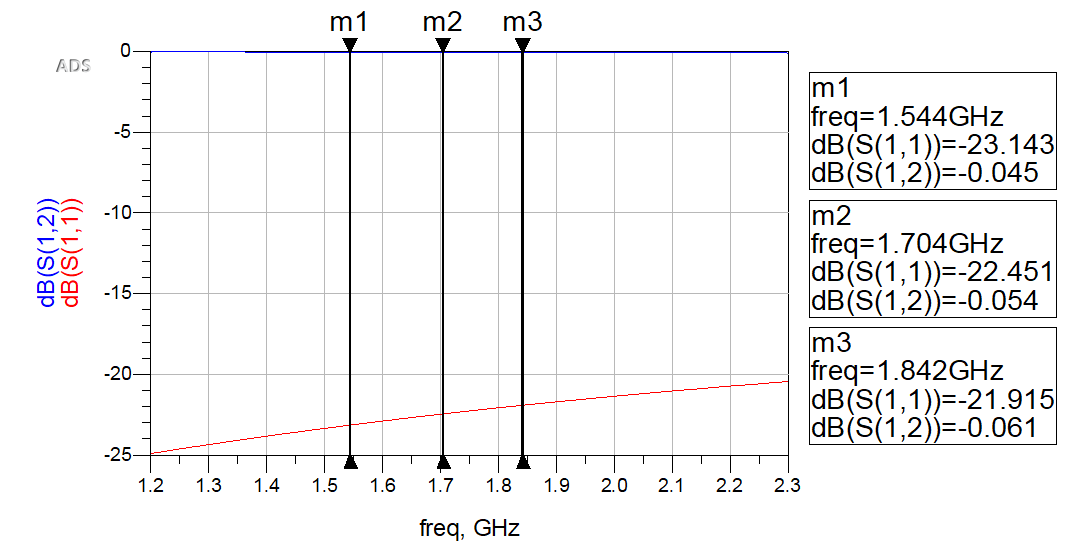
\includegraphics[width=0.75\linewidth]{imagenes/vcolay.png}
    \caption{Simulación del layout de la línea de transmisión CPWG de $50~\Omega$. (Fuente: propia).}
    \label{fig:vcolay}
\end{figure}

Por último, se obtuvo como resultado una impedancia de salida simulada y optimizada de $51~\Omega$.

\section{Construcción del bloque}

Una vez finalizado el diseño y verificados los parámetros de funcionamiento, se procedió a la construcción del bloque correspondiente al VCO. Para su implementación se utilizó una placa de FR-4 de dimensiones $30\times50~\mathrm{mm}$, sobre la cual se montaron el VCO y los elementos necesarios para su alimentación y conexión con el resto del sistema.

Los componentes utilizados para la construcción del bloque se resumen en la Tabla~\ref{tab:componentes_vco}.

\begin{table}[h]
\centering
\begin{tabular}{lc}
\hline
\textbf{Componente} & \textbf{Cantidad / Característica} \\
\hline
Placa de circuito impreso & FR-4, $30\times50~\mathrm{mm}$ \\
VCO & CVCO55BE-1530-2700 \\
Conector SMA & 2 \\
Capacitor de desacople & $0{,}1~\mu\mathrm{F}$ \\
Máscara de PCB & Pintura UV \\
\hline
\end{tabular}
\caption{Componentes utilizados para la construcción del bloque VCO.}
\label{tab:componentes_vco}
\end{table}

La placa cuenta con dos conectores SMA, destinados a la salida de RF y a la conexión de la tensión de sintonización ($V_{\text{tune}}$), respectivamente. La alimentación del VCO se realizó mediante un conector MTA conectado al terminal de $V_{CC}$ del dispositivo.

Para mejorar el ruido de la alimentación, se incorporó un capacitor de desacople de $0{,}1~\mu\mathrm{F}$ ubicado próximo al VCO. Este componente permite reducir las componentes de alta frecuencia presentes en la línea de alimentación y minimizar su influencia sobre el funcionamiento del oscilador.

Finalmente, se utilizó pintura UV como máscara para proteger las pistas y facilitar el proceso de fabricación de la placa. Una vez finalizado el montaje, se obtuvo el bloque físico del VCO, preparado para su integración con el resto del sistema de generación de chirp.

En la Figura~\ref{fig:placavco1} se muestra la placa desarrollada.

\begin{figure}[H]
    \centering
    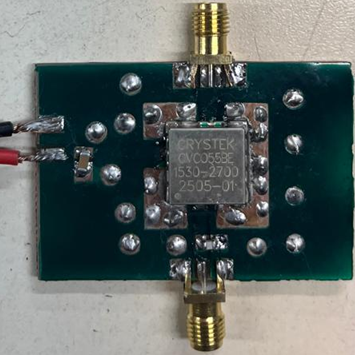
\includegraphics[width=0.5\linewidth]{imagenes/placavco.png}
    \caption{Placa del VCO desarrollada en el LARFyM. (Fuente: propia).}
    \label{fig:placavco1}
\end{figure}

\section{Medición}

Una vez finalizada la construcción del bloque VCO, se realizaron mediciones experimentales con el objetivo de verificar su comportamiento y comparar los resultados obtenidos con las especificaciones y estimaciones realizadas previamente.

Se realizaron mediciones de la tensión de sintonización ($V_{\text{tune}}$) para diferentes frecuencias de salida, con el objetivo de determinar experimentalmente la sensibilidad de sintonía del VCO ($K_V$). Además, se caracterizó el contenido espectral de la señal de salida mediante la medición de espurios.

En la Figura~\ref{fig:vcolazoabi} se muestra el VCO funcionando a lazo abierto con una tensión de control de $0~\mathrm{V}$ para evitar errores en la medición debido a ruido que ingrese por el pin de tensión de control.

\begin{figure}[H]
    \centering
    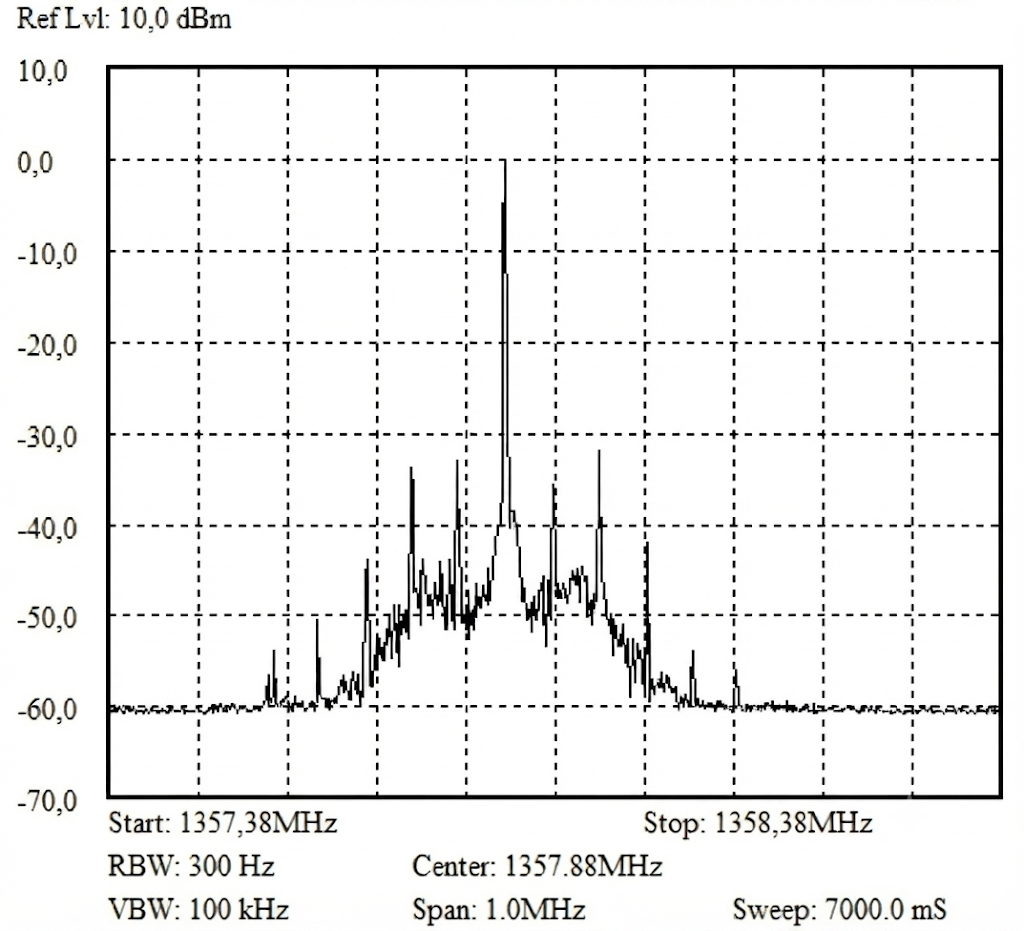
\includegraphics[width=0.5\linewidth]{imagenes/vcomedicionanalizador.png}
    \caption{Medición del VCO a lazo abierto. (Fuente: propia).}
    \label{fig:vcolazoabi}
\end{figure}

\subsection{Medición de la sensibilidad de sintonía}

Para determinar la sensibilidad de sintonía real del VCO, se midió la tensión de sintonización ($V_{\text{tune}}$) correspondiente a diferentes frecuencias de salida. Los resultados obtenidos se presentan en la Tabla~\ref{tab:kv_real}.

\begin{table}[htbp]
\centering
\begin{tabular}{lc}
\hline
\textbf{Frecuencia} & \textbf{$V_{\text{tune}}$ medido} \\
\hline
$1550~\mathrm{MHz}$ & $1{,}19~\mathrm{V}$ \\
$1587{,}5~\mathrm{MHz}$ & $1{,}45~\mathrm{V}$ \\
$1625~\mathrm{MHz}$ & $1{,}69~\mathrm{V}$ \\
$1662{,}5~\mathrm{MHz}$ & $1{,}935~\mathrm{V}$ \\
$1700~\mathrm{MHz}$ & $2{,}238~\mathrm{V}$ \\
$1737{,}5~\mathrm{MHz}$ & $2{,}436~\mathrm{V}$ \\
$1775~\mathrm{MHz}$ & $2{,}67~\mathrm{V}$ \\
$1812{,}5~\mathrm{MHz}$ & $2{,}89~\mathrm{V}$ \\
$1850~\mathrm{MHz}$ & $3{,}15~\mathrm{V}$ \\
\hline
\end{tabular}
\caption{Valores experimentales de tensión de sintonización del VCO.}
\label{tab:kv_real}
\end{table}

En la Figura~\ref{fig:medicionrampa} se presenta la rampa de frecuencia generada por el VCO en ausencia del PLL. Se incluye, además, la comparación con la rampa de frecuencia ideal correspondiente al barrido requerido y la desviación respecto de esta última. Esta comparación permite cuantificar el error introducido por las no idealidades del VCO y evaluar la necesidad de incorporar el PLL y su filtro de lazo para corregir dichas desviaciones y obtener un barrido de frecuencia más próximo al comportamiento ideal.

\begin{figure}[H]
    \centering
    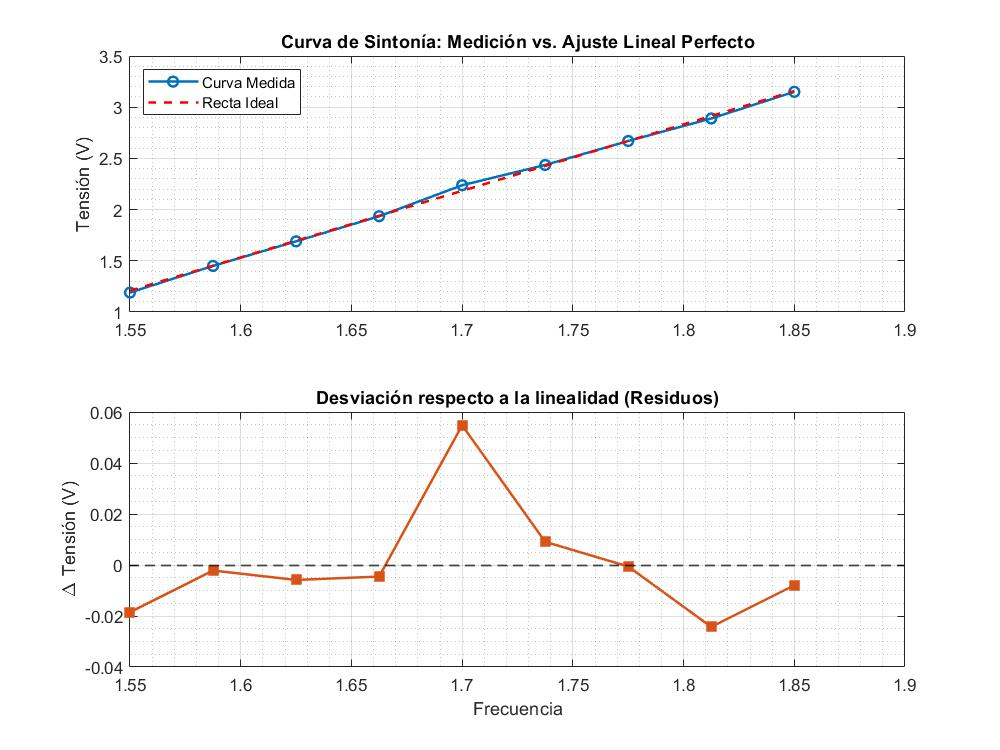
\includegraphics[width=0.75\linewidth]{imagenes/rampanolinealyerror.jpg}
    \caption{Comparación entre la rampa medida y la ideal. (Fuente: propia).}
    \label{fig:medicionrampa}
\end{figure}

A partir de los valores extremos de la tabla se calculó la sensibilidad de sintonía promedio del VCO mediante:

\begin{equation}
K_V = \frac{\Delta f}{\Delta V_{\text{tune}}}.
\end{equation}

La variación de frecuencia medida fue:

\begin{equation}
\Delta f = 1850 - 1550 = 300~\mathrm{MHz},
\end{equation}

mientras que la variación correspondiente de la tensión de sintonización resultó:

\begin{equation}
\Delta V_{\text{tune}} = 3{,}15 - 1{,}19 = 1{,}96~\mathrm{V}.
\end{equation}

Por lo tanto, la sensibilidad de sintonía experimental obtenida fue:

\begin{equation}
K_{V,\mathrm{exp}} = \frac{300~\mathrm{MHz}}{1{,}96~\mathrm{V}} \approx 153{,}06~\mathrm{MHz/V}.
\end{equation}

Este resultado puede compararse con el valor obtenido previamente a partir de la hoja de datos, de aproximadamente $142{,}86~\mathrm{MHz/V}$.

La diferencia observada puede atribuirse a la dispersión propia del componente, a las tolerancias de los elementos utilizados y a las condiciones de medición, además de las aproximaciones asociadas a la lectura de la curva proporcionada por el fabricante. Por otro lado, la hoja de datos no asegura que el VCO tenga la misma sensibilidad $K_V$ a lo largo de todo su rango de frecuencias.

\subsection{Medición de espurios}
Se realizó la caracterización espectral de la señal de salida del VCO mediante un analizador de espectro. La componente principal corresponde a la frecuencia de oscilación del VCO, mientras que las componentes de menor amplitud corresponden a señales espurias presentes alrededor de la portadora. Estos son complejos de mitigar debido a que el responsable de generarlos es el propio VCO; como indica \cite{Dean Banerjee}, es la causa más complicada de disminuir y no tendrán gran impacto siempre y cuando el PLL no los confunda con la señal a sintonizar.

El nivel de los espurios se expresa relativo a la potencia de la portadora, en unidades de dBc, mediante:

\begin{equation}
S_{\mathrm{spur}} = P_{\mathrm{spur}} - P_{\mathrm{carrier}} = -32~\mathrm{dBc}.
\end{equation}

A partir del espectro obtenido se identificaron las principales componentes espurias y se determinó su nivel relativo respecto de la portadora.

\subsection{Ruido de fase}

Se realizó la medición del ruido de fase del VCO para una frecuencia de salida fija, con el objetivo de caracterizar la estabilidad espectral y compararla con la señal generada por el PLL. El resultado obtenido experimentalmente se presenta en la Figura~\ref{fig:ruido_fase_vco}.

\begin{figure}[H]
    \centering
    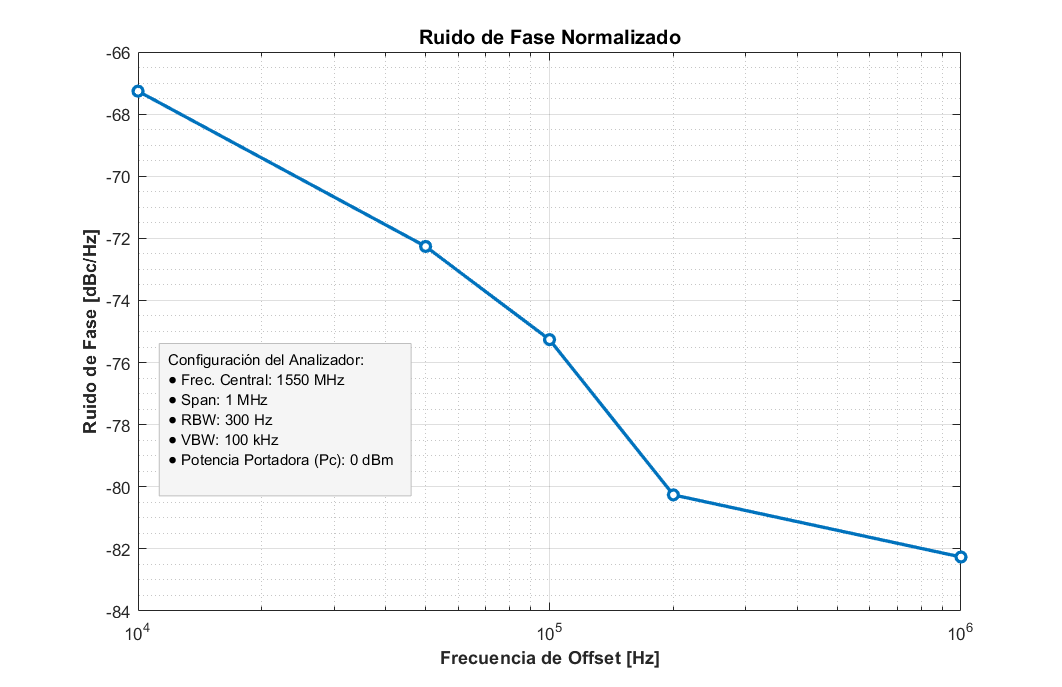
\includegraphics[width=0.85\textwidth]{imagenes/ruido_fase_vco.png}
    \caption{Medición del ruido de fase del VCO a frecuencia fija. (Fuente: propia).}
    \label{fig:ruido_fase_vco}
\end{figure}